%!TEX root = ../../thesis.tex
\section{Three-way merges}
\label{sync-3waymerges}

\begin{figure}[htb]
  \centerline{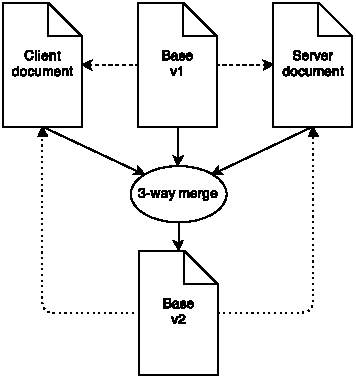
\includegraphics[width=0.55\linewidth]{images/Three-way_merge.pdf}}
  \caption[Illustration of a three-way merge - based upon
  \protect\newline{\small\url{https://neil.fraser.name/writing/sync/3way.gif} (02.5.2014)}
  \protect\newline{\small\emph{Neil Frasier}}]{Illustration of a three-way merge}
  \label{fig:Threewaymerge}
\end{figure}

Three-way merges are commonly used in many source code management systems, e.g. in git \cite[p. 52]{scott2009pro} or in CVS \cite[p. 31f]{lindholm2001athreeway}. Their purpose is to allow users to work on the same files simultaneously without necessitating a constant connection to a server. The way a three-way merge works is illustrated in \reffigure{fig:Threewaymerge}. The algorithm takes the changed local version of the document, its base version and the changed server document (that is also based upon the same document as the client's). It then compares the changes that were made to both new documents, in comparison to the base version \cite[p. 2f]{mens2002softwaremerging}. These changes are then merged into a new version of the document, on which all subsequent changes have to be built on top of. Sometimes not all changes can be merged into a new version automatically e.g. because both changed versions have alterations to the same part of the document. This results in a conflict that can only be resolved manually by the user, which is one of the reasons why three-way merges are often executed on the client.

This approach can also be used for real-time collaborative editing by permitting clients to send their new versions of the document to the server, which then performs a three-way merge and returns the newly generated base document or the list of conflicts that the user needs to resolve \cite[p. 220ff]{minor1993semiasynchronous}. In this way, all users could edit the same document(s) simultaneously. Since all edits are done locally and all conflicts need to be resolved manually, this algorithm ensures that Convergence, Intention Preservation and Causality preservation are achieved. Furthermore, it complies with the UX requirements: \textbf{Graceful Exit} (manual conflict resolution) and \textbf{Full Concurrency} (documents are not locked). 

One major drawback to this technique is that it is poor at Latency Hiding. This is due to the fact that no updated document can be sent to the server while the user is editing. Once the user has finished, an updated version can be sent and merged but if the document has been updated during the merge, the merged version cannot be applied and needs to be revoked \cite[p. 2]{fraser2009differential}. This behavior results in versions that will diverge more over time, thus generating a higher chance for merge conflicts and merge conflicts require user interaction. Having to deal with merge conflicts instead of being able to focus efforts on working on the document has a bad impact on the user experience.

In addition to this, the algorithm does not scale well for larger documents, as the whole document needs to be transferred to the server for each merge. Also it does not scale in scenarios with many connected users. This is due to the problem that having more simultaneous users in a system, the chances of merge conflicts rise.